
\section{Proof of Theorem~\ref{t:main}} \label{s:proof}

To aid readability of the relatively long proof of this theorem we split it into four lemmas.
We start with some notation.

\begin{definition}
	Let $\P_q(n)$ be the set of all sets $U = \{u_1 < \cdots < u_{n-i}\}$ with $u_j \in \{0, \dots, n\}$.
	For any $U \in \P_q(n)$, let $\overline{U} \in \P_{n+1-q}(n)$ contain the elements of $\{0, \dots, n\}$ not in $U$. For $x \in \overline{U}$, define $x.U \in \P_{q+1}(n)$ to contain $x$ and the elements in $U$.
	For $x \in U$, define $U \setminus x \in \P_{q-1}(n)$ to contain the elements in $U$ different from $x$.
\end{definition}

Recall that for any $U = \{u_1 < \cdots < u_q\} \in \P_q(n)$ we write $d_U$ for $d_{u_1}^{n-q+1} \cdots \,d_{u_q}^n$ and avoid writing the superscripts when they do not contribute to expositional clarity.
With this notation we have for any $x \in X_n$
\begin{equation*}
\Delta_{n-q}(x)\ =\! \sum_{U \in \P_q(n)} d_{U^+}(x) \otimes d_{U^-}(x).
\end{equation*}

\begin{lemma} \label{l:partial dU = dxU}
	For any $x \in X_n$ and $U \in \P_{q}(n)$
	\begin{equation} \label{lemma1: existence: eq1}
	\partial \circ d_U(x) = \sum_{\bar{u} \in \overline{U}} d_{\bar{u}.U}(x).
	\end{equation}
\end{lemma}

\begin{proof}
	Let $U = \{u_1 < \cdots < u_q\}$. Using the simplicial relation \eqref{e:simplicial relation} we have
	\begin{equation*}
	\partial \circ d_U(x) = 
	\sum_{i=0}^{n-q} d_i\, d_{u_1} \cdots\, d_{u_q}(x) = 
	\sum_{\bar{u} \in \overline{U}} d_{u_1} \cdots\, d_{\bar{u}} \cdots\, d_{u_q}(x) =
	\sum_{\bar{u} \in \overline{U}} d_{\bar{u}.U}(x)
	\end{equation*}
	as claimed.
\end{proof}

\anibal{Check the $q=0$ case below.}

\begin{lemma} \label{l:pigeon hole}
	For any $x \in X_n$ and $q \in \{0, \dots, n\}$
	\begin{equation} \label{e:pigeon hole 1}
	\Delta_{n-q-1} \circ \partial (x)\ =\! 
	\sum_{U \in \P_q(n)} \left( 
	\sum_{u \in U^-} d_{u.U^+}(x) \tensor d_{U^-}(x) + 
	\sum_{u \in U^+} d_{U^+}(x) \tensor d_{u.U^-}(x) \right).
	\end{equation}
\end{lemma}

\begin{proof}
	Let
	\begin{align*}
	& S_1 = \big\{ (u, V)\ |\ V \in \P_{q-1}(n-1) \text{ and } u \in \{0,\dots,n\} \big\}, \\
	& S_2 = \big\{ (w, W)\ |\ W \in \P_{q}(n) \text{ and } w \in W \big\}
	\end{align*}
	and notice that identity \eqref{e:pigeon hole 1} is equivalent to the following identity:
	\begin{equation} \label{e:pigeon hole 2}
	\sum_{(u, V) \in S_1} d_{V^+}d_u \tensor d_{V^-}d_u \ \, = \!
	\sum_{(w, W) \in S_2} 
	\begin{cases}
	d_{w.W^+} \tensor d_{W^-} & \text{ if } w \in W^-, \\
	d_{W^+} \tensor d_{w.W^-} & \text{ if } w \in W^+.
	\end{cases}
	\end{equation}	
	Define $S_1 \to S_2$ by sending $\big(u,\, \{v_1 < \cdots < v_{q-1}\} \big)$ to $\big(u,\, \{w_1 < \cdots < w_{q}\} \big)$ with
	\begin{equation*}
	w_i = 
	\begin{cases}
	v_i & \text{ if } v_i < u, \\
	u & \text{ if } v_i < u \leq v_{i+1}, \\
	v_{i-1}+1 & \text{ if } v_i < u.
	\end{cases}
	\end{equation*} 
	This function is a bijection since it is injective and both sets have cardinality 
	\begin{equation*}
	\frac{(n+1)!}{(n+1-q)!(q-1)!}.
	\end{equation*}
	To establishes \eqref{e:pigeon hole 2} we use the simplicial identity to notice that if $(u, V) \mapsto (u, W)$ then
	\begin{equation*}
	d_{V^+}d_u \tensor d_{V^-}d_u =
	\begin{cases}
	d_{u.W^+} \tensor d_{W^-} & \text{ if } u \in W^-, \\
	d_{W^+} \tensor d_{u.W^-} & \text{ if } u \in W^+,
	\end{cases}
	\end{equation*}
	which concludes the proof.
\end{proof}


\begin{lemma} \label{l:boundary of Delta}
	For any $x \in X_n$ and $q \in \{0, \dots, n\}$
	\begin{equation} \label{e:boundary of Delta}
	\Big( \partial_{2n-q} \circ \Delta_{n - q} \, +\, \Delta_{n-q-2} \circ \partial_n \Big) (x) \ = \! 
	\sum_{\substack{U \in \P_{q}(n) \\ \bar u \in \overline{U}}} \Big( d_{\bar u.U^+} \tensor d_{U^-} \, + \, d_{U^+} \tensor d_{\bar u.U^-} \Big) (x \otimes x).
	\end{equation}
\end{lemma}

\begin{proof}
	Using Lemma~\ref{l:partial dU = dxU} and Lemma~\ref{l:pigeon hole} we have
	\begin{equation*}
	\begin{split}
	\partial_{2n-q} \circ \Delta_{n - q} (x) \ = & \
	\sum_{U \in \P_q(n)} \Big( \partial \circ d_{U^+} \tensor d_{U^-}\ +\ d_{U^-} \tensor \partial \circ d_{U^-} \Big) (x \otimes x) \\ = & \!\!
	\sum_{\substack{U \in \P_q(n) \\ v \in \overline{U^+},\ w \in \overline{U^-} } }\!\! \Big( d_{v.U^+} \tensor d_{U^-}\ +\ d_{U^+} \tensor d_{w.U^-}\Big) (x \otimes x) \\ = &
	\quad \Delta_{n-q-2} \circ \partial_n (x) \ + 
	\sum_{\substack{U\in\P_{q}(n) \\ \bar u \in \overline{U}}} \Big( d_{\bar u.U^+} \tensor d_{U^-}\ +\ d_{U^+} \tensor d_{\bar u.U^-}\Big) (x \otimes x)
	\end{split}
	\end{equation*}
	as claimed.
\end{proof}

\begin{lemma} \label{l:large lemma}  
	For any $x \in X_n$ and $q \in \{0, \dots, n\}$
	\begin{equation} \label{lemma4: existence: eq1}
	\sum_{\substack{U \in \P_{q}(n) \\ x \in \overline{U}}} d_{x.U^-} \tensor d_{U^+}\ +\ d_{U^-} \tensor d_{x.U^+}\ = \
	(1+T) \sum_{U \in \P_{q+1}(n)} d_{U^-} \tensor d_{U^+.}
	\end{equation}
\end{lemma}

\textit{Proof.}
For $U = (u_1, \dots, u_q) \in \P_{q}(n)$ define when possible:\\
\begin{minipage}{.5\textwidth}
	\begin{align*}
	& l_{U,x} = \max\{u\in U\ |\ x>u\} \\
	& V_{U,x} = (v_1, \dots v_q) \text{ with }
	v_i = 
	\begin{cases}
	u_i & \text{ if } u_i \neq l_{U,x} \\
	x	& \text{ if } u_i = l_{U,x}
	\end{cases}
	\end{align*} 
\end{minipage}
\begin{minipage}{.5\textwidth}
	\begin{align*}
	& r_{U,x} = \min\{u\in U\ |\ x<u\} \\
	& W_{U,x} = (w_1, \dots w_q) \text{ with }
	w_i = 
	\begin{cases}
	u_i & \text{ if } u_i \neq r_{U,x} \\
	x	& \text{ if } u_i = r_{U,x}.
	\end{cases}
	\end{align*}
\end{minipage}\\ \\
Notice that $(l_{U,x}).V_{U,x} = x.U = (r_{U,x}).W_{U,x}$ and that for any $u \in x.U$ with $u \neq l_{U,x},\, x,\, r_{U,x}$ we have $\ind_{V_{U,x}}(u) = \ind_{U}(u) = \ind_{W_{U,x}}(u)$.

We introduce the following sets using tabbing and a schematic to aid readability: \\

\begin{minipage}{.3\textwidth}
	\begin{center}
		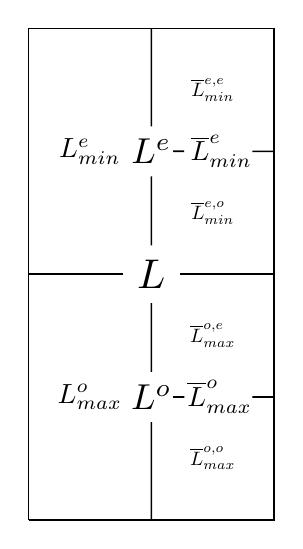
\begin{tikzpicture}[scale = .26]
		\node (L) at (0,0) [scale = 1.5]{$L$};
		\draw [semithick] (-6,0) -- (L) -- (6,0);
		\draw [semithick] (-6,-12) -- (6,-12) -- (6,12) -- (-6,12) -- (-6,-12);
		Statement
		\node (Le) at (0,6) [scale = 1.3] {$L^e$};
		\node (Lemax) at (-3,6) {$ {L}^e_{min}$};
		\node (-Lemax) at (3,6) {$\; \overline{L}^e_{min}$\!\!};
		\node at (3,3) [scale = .7] {$\overline{L}^{e,o}_{min}$};
		\node at (3,9) [scale = .7] {$\overline{L}^{e,e}_{min}$};
		
		\draw [semithick] (L) -- (Le) -- (0,12);
		\draw [semithick] (6,6) -- (-Lemax) -- (Le);
		
		\node (Lo) at (0,-6) [scale = 1.3] {$L^o$};
		\node (Lomin) at (-3,-6) {$ {L}^o_{max}$};
		\node (-Lomin) at (3,-6) {$\, \overline{L}^o_{max}$\!\!};
		\node at (3,-3) [scale = .7] {$\overline{L}^{o,e}_{max}$};
		\node at (3,-9) [scale = .7] {$\overline{L}^{o,o}_{max}$};
		
		\draw [semithick] (L) -- (Lo) -- (0,-12);
		\draw [semithick] (6,-6) -- (-Lomin) -- (Lo);
		\end{tikzpicture}
	\end{center}
\end{minipage}
\begin{minipage}{.8\textwidth}
	$L = \{x.U^- \tensor U^+\ | \ U \in \P_q(n),\ x \in \overline{U}\}$. \\
	\begin{tab}
		$L^{e} = \{x.U^- \tensor U^+ \in L\ | \ \ind_{x.U}(x) \text{ even}\}$. 
		\begin{tab}
			$L_{min}^{e} = \{x.U^- \tensor U^+ \in L^e\ | \ x < u_1 \}$.\par
			$\overline{L}_{min}^{e} = L^{e} \setminus L_{min}^{e}$.
			\begin{tab}
				$\overline{L}_{min}^{e,e} = \{ x.U^- \tensor U^+ \in \overline{L}_{min}^{e}\ | \ \ind_{x.U}(l_{U,x}) \text{ even} \}$.\par
				$\overline{L}_{min}^{e,o} = \{ x.U^- \tensor U^+ \in \overline{L}_{min}^{e}\ | \ \ind_{x.U}(l_{U,x}) \text{ odd} \}.$ \\
			\end{tab}
		\end{tab}
		$L^{o} = \{x.U^- \tensor U^+\ | \ \ind_{x.U}(x) \text{ odd}\}$.\par 
		\begin{tab}
			$L_{max}^{o} = \{x.U^- \tensor U^+ \in L^o\ | \ u_q < x \}$.\par
			$\overline{L}_{max}^{o} = L^{o}\setminus L_{max}^{o}$.
			\begin{tab}
				$\overline{L}_{max}^{o,e} = \{ x.U^- \tensor U^+ \in \overline{L}_{max}^{o}\ | \ \ind_{x.U}(r_{U,x}) \text{ even} \}$.\par 
				$\overline{L}_{max}^{o,o} = \{ x.U^- \tensor U^+ \in \overline{L}_{max}^{o}\ | \ \ind_{x.U}(r_{U,x}) \text{ odd} \}$.
			\end{tab}
		\end{tab}
	\end{tab}
\end{minipage}

\begin{minipage}{.3\textwidth}
	\begin{center}
		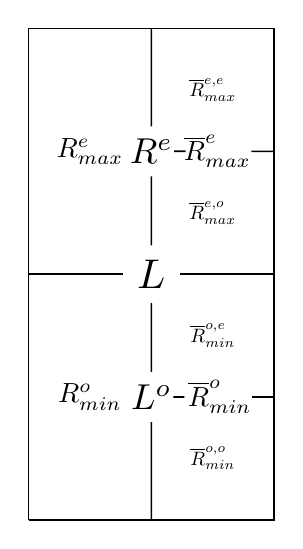
\begin{tikzpicture}[scale = .26]
		\node (L) at (0,0) [scale = 1.5]{$L$};
		\draw [semithick] (-6,0) -- (L) -- (6,0);
		\draw [semithick] (-6,-12) -- (6,-12) -- (6,12) -- (-6,12) -- (-6,-12);
		
		\node (Le) at (0,6) [scale = 1.3] {$R^e$};
		\node (Lemax) at (-3,6) {$ {R}^e_{max}$};
		\node (-Lemax) at (3,6) {$\overline{R}^e_{max}$\!\!};
		\node at (3,3) [scale = .7] {$\overline{R}^{e,o}_{max}$};
		\node at (3,9) [scale = .7] {$\overline{R}^{e,e}_{max}$};
		
		\draw [semithick] (L) -- (Le) -- (0,12);
		\draw [semithick] (6,6) -- (-Lemax) -- (Le);
		
		\node (Lo) at (0,-6) [scale = 1.3] {$L^o$};
		\node (Lomin) at (-3,-6) {$ {R}^o_{min}$};
		\node (-Lomin) at (3,-6) {\,$\overline{R}^o_{min}$\!\!};
		\node at (3,-3) [scale = .7] {$\overline{R}^{o,e}_{min}$};
		\node at (3,-9) [scale = .7] {$\overline{R}^{o,o}_{min}$};
		
		\draw [semithick] (L) -- (Lo) -- (0,-12);
		\draw [semithick] (6,-6) -- (-Lomin) -- (Lo);
		\end{tikzpicture}
	\end{center}
\end{minipage}
\begin{minipage}{.8\textwidth}
	$R = \{U^-\tensor x.U^+\ | \ U \in \P_q(n),\ x \in \overline{U}\}$.\\
	\begin{tab}
		$R^{e} = \{U^-\tensor x.U^+ \in R\ | \ \ind_{x.U}(x) \text{ even}\}$.\par
		\begin{tab}
			$R_{max}^{e} = \{U^- \tensor x.U^+ \in R^e\ | \ u_q < x \}$.\par 
			$\overline{R}_{max}^{e} = R^{e} \setminus R_{max}^{e}$.
			\begin{tab}
				$\overline{R}_{max}^{e,e} = \{ U^- \tensor x.U^+ \in \overline{R}_{max}^{e}\ | \ \ind_{x.U}(r_{U,x}) \text{ even} \}$.\par 
				$\overline{R}_{max}^{e,o} = \{ U^- \tensor x.U^+ \in \overline{R}_{max}^{e}\ | \ \ind_{x.U}(r_{U,x}) \text{ odd} \}$.\\
			\end{tab}
		\end{tab}
		$R^{o} = \{U^- \tensor x.U^+ \in R\ | \ \ind_{x.U}(x) \text{ odd}\}$.\par 
		\begin{tab}
			$R_{min}^{o} = \{U^- \tensor x.U^+ \in R^o \ | \  x < u_1 \}$.\par 
			$\overline{R}_{min}^{o} = R^{o} \setminus R_{min}^{o}$.
			\begin{tab}
				$\overline{R}_{min}^{o,e} = \{ U^- \tensor x.U^+ \in \overline{R}_{min}^{o}\ | \ \ind_{x.U}(l_{U,x}) \text{ even} \}$.\par 
				$\overline{R}_{min}^{o,o} = \{ U^- \tensor x.U^+ \in \overline{R}_{min}^{o}\ | \ \ind_{x.U}(l_{U,x}) \text{ odd} \}$.
			\end{tab}
		\end{tab}
	\end{tab}
\end{minipage} \\ \\
We claim the following four identities: 
\begin{equation}\label{lemma4: existence: eq2}
\overline{R}_{min}^{o,o} = \overline{L}_{max}^{o,o}\ , \qquad \overline{R}_{min}^{o,e} = \overline{R}_{max}^{e,o}\ , \qquad 
\overline{L}_{min}^{e,o} = \overline{L}_{max}^{o,e}\ , \qquad \overline{L}_{min}^{e,e} = \overline{R}_{max}^{e,e}.
\end{equation}
We show only the proof of the first one. The other three are proven analogously.
\begin{alignat*}{2}
&\boxed{U^-\tensor x.U^+ \in \overline{R}_{min}^{o,o}}\ &\Longrightarrow\ &\boxed{U^-\tensor x.U^+ =\, l_{U,x}.V_U(x)^-\tensor V_{U,x}^+ \in \overline{L}_{max}^{o,o} \ \ } \\ 
&\boxed{x.U^-\tensor U^+ \in \overline{L}_{max}^{o,o}}\ &\Longrightarrow\ &\boxed{x.U^-\tensor U^+ =\, W_U(x)^-\tensor r_{U,x}.W_{U,x}^+ \in \overline{R}_{min}^{o,o} \! }
\end{alignat*}
The identities in (\ref{lemma4: existence: eq2}) imply 
\begin{equation} \label{lemma4: existence: eq3} 
\sum_{\overline{L}_{max}^{o}} d_{x.U^-} \tensor d_{U^+}\ \ +\ \ 
\sum_{\overline{R}_{max}^{e}} d_{U^-} \tensor d_{x.U^+}\ \ +\ \ 
\sum_{\overline{L}_{min}^{e}} d_{x.U^-} \tensor d_{U^+}\ \ +\ \ 
\sum_{\overline{R}_{min}^{o}} d_{U^-} \tensor d_{x.U^+} = 0.
\end{equation}
Let us now consider the right hand side of (\ref{lemma4: existence: eq1})
\begin{equation*}
\sum_{U\in\P_{q+1}(n)} d_{U^-} \tensor d_{U^+} +\, d_{U^+} \tensor d_{U^-.}
\end{equation*}
Notice it is equal to
\begin{align*}
&\, \sum_{\substack{U \in \P_{q+1}(n) \\ \ind_U(u_{q+1}) \text{ odd}}} d_{u_{q+1}.(U \smallsetminus u_{q+1})^-} \tensor d_{(U \smallsetminus u_{q+1})^+}\ \ + 
\sum_{\substack{U \in \P_{q+1}(n) \\ \ind_U(u_{q+1}) \text{ even}}} d_{(U\smallsetminus u_{q+1})^-} \tensor d_{u_{q+1}.(U \smallsetminus u_{q+1})^+}\ \ + \\
&\ \,\sum_{\substack{U \in \P_{q+1}(n) \\ \ind_U(u_1) \text{ even}}} d_{u_1.(U\smallsetminus u_1)^-} \tensor d_{(U\smallsetminus u_1)^+}\ \ +
\sum_{\substack{U \in \P_{q+1}(n) \\ \ind_U(u_1) \text{ odd}}} d_{(U \smallsetminus u_1)^-} \tensor d_{u_1.(U\smallsetminus u_1)^+.}
\end{align*}
This expression, in turn, equals
\begin{equation*} 
\sum_{{L}_{max}^{o}} d_{x.U^-} \tensor d_{U^+}\ \ +\ \ 
\sum_{{R}_{max}^{e}} d_{U^-} \tensor d_{x.U^+}\ \ +\ \ 
\sum_{{L}_{min}^{e}} d_{x.U^-} \tensor d_{U^+}\ \ +\ \ 
\sum_{{R}_{min}^{0}} d_{U^-} \tensor d_{x.U^+.}
\end{equation*}
Thanks to (\ref{lemma4: existence: eq3}), the above expression equals
\begin{equation*}
\sum_{L} d_{x.U^-} \tensor d_{U^+}\ +\ \ 
\sum_{R} d_{U^-} \tensor d_{x.U^+,}
\end{equation*}
the left hand side of (\ref{lemma4: existence: eq1}).

The proof of Proposition \ref{proposition: chain map}, the chain map property, now follows directly from Lemma \ref{lemma3: existence} and Lemma \ref{lemma4: existence}.